%main

\documentclass{article}

\usepackage{geometry} \usepackage{graphicx}
\usepackage{amsmath}
\usepackage{listings}
\usepackage{multirow}
\usepackage{fancyhdr}

\pagestyle{fancy}
\fancyhf{}
\rhead{Dine Elreedy, Chen Liu, Hang Yan, Hao Yan}
\lhead{CSE 427 Final Project Report}

\title{CSE 427 final project report\\
  Netflix user rating prediction with collaborative filtering}

\author{Dina Elreedy, Chen Liu, Hang Yan, Hao Yan}

\begin{document}
\maketitle
  \section{Introduction}
  In this project we tackled the problem of predicting the ratings for
  movies, which can be helpful for recommender systems by recommending movies of high predicted ratings by a user to him. Formally, given a set of $n$ users and $k$ movies and an
  incomplete rating matrix $U$ of $n$ by $k$ entries, our task is to predict the
  missing entries of $U$. The prediction is made possible with a large
  set of training data, consisting the incomplete rating of other $m$
  users for the same set of $k$ movies.

  There are multiple ways to solve this problem. The algorithm we are
  using is collaborative filtering, which takes the idea from $kth$
  nearest neighbor search (KNN). Given a user and the movie whose
  rating we want to predict, we first find similar users in the
  training set that have the ratings on this movie, then predict the
  unknown rating from these known ratings. The core of the algorithm is
  to find similar users with the testing user in the training
  set. Given the scale of the problem, we implemented our algorithm
  with MapReduce and execute it on the real cloud platform.

  %Write about analysis and preprocessing here
\section{Data analysis}
The data we use is a subset of Netflix Prize data. The data consists
of ratings for 17770 movies. There are ratings from 3255352 users in
the training set and 100478 users in the tests set (numbers computed
from the line count of TrainingRatings.txt, TestingRatings.txt and
movie\_titles.txt). The size of the problem indicates that cloud
computing is necessary.

For a better algorithm design, we first performed analysis to the
dataset with Spark. A random subset of the data is drawn for the
analysis, see Table~\ref{tab:subsample} for the size of sampled
data. The analysis gives us the answer of the following problems:

\begin{table}
  \centering
  \begin{tabular}{| p{5cm} | p{3cm} | p{3cm} |}
      \hline
       & Movie & User \\
      \hline
      Training set & 1821 & 28978\\
      \hline
      Testing set & 1701 & 27555\\
      \hline
  \end{tabular}
  \caption{The size of sampled data for analysis}
  \label{tab:subsample}
\end{table}

\subsection*{Similarity measurement}
The first key design choice is which similarity measurement to use for
the $kth$ nearest neighbor search. To this end, we compute the
histogram of average user ratings in the training set, see
Figure~\ref{fig:hist}.
\begin{figure}[!ht]
  \centering
  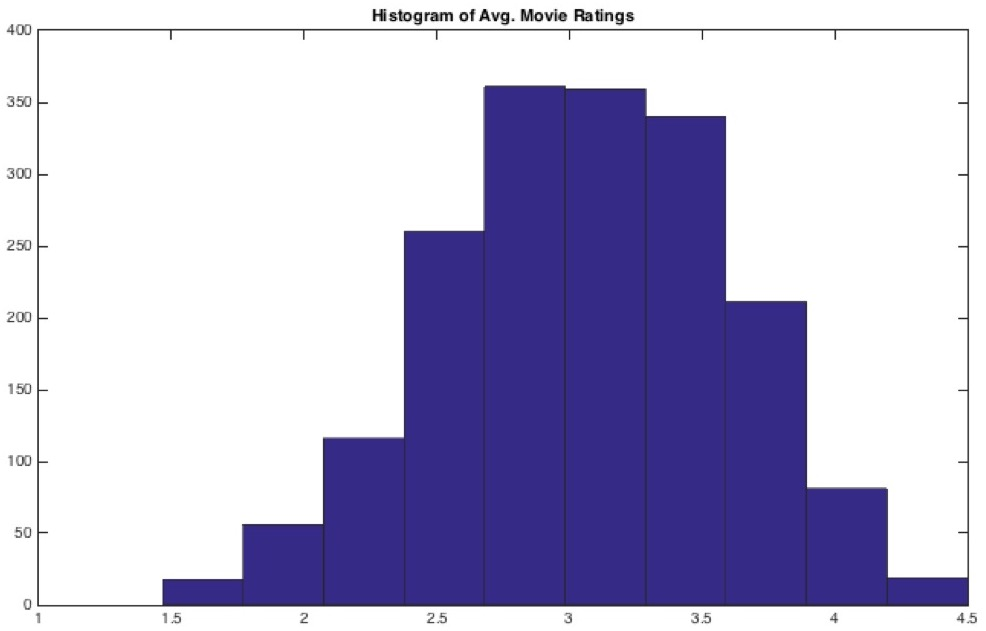
\includegraphics[width=0.9\textwidth]{images/hist}
  \caption{Histogram of average user ratings in the training set}
  \label{fig:hist}
\end{figure}

The result suggests that most users rate normally. Therefore, we
choose to use cosine similarity rather than Pearson similarity for
efficiency.

\subsection*{User-user similiary vs. movie-movie similarity}
To fill the missing entry, we can either use user as the key and fill with
ratings of other similar users, or we can use movie as the key and
fill with ratings of other similar movies. The choice depends of the
expected overlay of users in test and train and items in test and
train. See Table~\ref{tab:overlay}.

\begin{table}[!ht]
  \centering
  \begin{tabular}{|p{5cm}|p{5cm}|}
    \hline
    user-user & movie-movie\\
    \hline
    0.125467 & 0.439962\\
    \hline
  \end{tabular}
  \caption{Expected overly of two different keys}
  \label{tab:overlay}
\end{table}

The result suggests that use movie-movie similarity is more
appropriate.

\subsection*{Memory consumption}
The algorithm will use two MapReduce jobs: the first job computes
the list of users that rate each movie, and the second job computes
the similarity of each pair of movies. The memory bottleneck happens
at the reducer of each job. For first job, the expected memory usage
is 111.5589MB and for the second job, the expected memory usage is 4.4MB.

To summarize, given a user with missing ratings, we predict those
missing ratings one by one. For each movie whose rating is missing
(the query movie), the algorithm first computes movies that have
similar user ratings with the query movie, then predicts the missing
rating with known ratings from the similar movies. The similarity is
measured by Cosine similarity.

    
  %Write about collaboarative filter here
\section{Implementation}
Our algorithm mainly consists of two stages: the first stage is finding the most similar movies for each movie in the test set based on their overlapping ratings and the second stage is predicting the corresponding missing entries of the ratings matrix $U$ for pairs in the test set.

For the first stage, we have implemented it using three map reduce jobs:\\
\begin{itemize}
\item  Job1:
This job works on the training set, it produces movie-movie pairs and their ratings by each user.\\
Mapper Input:($movie_i$,$user_k$,$rate_{ik}$) triplets\\
Mapper Output:($user_k$,($movie_i$,$rate_ik$))\\
Reducer Input:($user_k$,[($movie_1$,$rate_1k$),..($movie_i$,$rate_ik$),...]), all movies rated by user k along with their rates\\
Reducer Output:($movie_i$,$movie_j$),($rate_{jk}$,$rate_{jk}$), all pairs of movies rated by user k and their rates \\
\item Job2:
This job works on the first job's output, the job mainly calculates cosine similarity between every pair of movies provided in the first job's output using their overlapped ratings.\\ 
Mapper Input:($movie_i$,$movie_j$),($rate_{ik}$,$rate_{jk}$), rated pairs by user k.\\
Mapper Output: ($movie_i$,$movie_j$),($rate_{ik}$,$rate_{jk}$) (It is Identity Mapper)\\
Reducer Input:($movie_i$,$movie_j$),[($rate_{i1}$,$rate_{j1}$),($rate_{i2}$,$rate_{j2}$),...($rate_{ik}$,$rate_{jk}$)])\\
Reducer Output:($movie_i$,$movie_j$),$cos_sim(movie_i,movie_j)$\\
\item Job3:
After calculating similarity between each movie pairs, the third job selects the top-k similar movies for each movie. The default $K$ we use is 10, however, we can pass K as an input parameter using command line.\\
Mapper Input:(($movie_i$,$movie_j$),$cos_sim(movie_i,movie_j)$\\
Mapper Output:($movie_i$,($movie_j,cos_sim(movie_i,movie_j)$)\\
Reducer Input:($movie_i,[(movie_j,cos_sim(movie_i,movie_j$),.($movie_k,cos_sim(movie_i,movie_k),....]$), list of all overlapped movies with $movie_i$and their corresponding rates\\
Reducer Output:Top-K similar movies per movie $i$: $(movie_i,[(movie_j,cos_sim(movie_i,movie_j),.(movie_k,cos_sim(movie_i,movie_k)])$\\
\end{itemize}

For the second stage, since the top-K entries per movie is a small number, then this task does not require a Map Reduce job. Accordingly, we have implemented it using....


  %Write about cloud execution here
\section{Cloud execution}


  %Write result here
\section{Results}
We evaluated the performance of our algorithm and the impact of
parameters on a subset of Netflix Prize dataset by the prediction
accuracy and the number of unpredicted ratings in the test set. We
report two accuracy measurements: the root mean swuare error(RMSE) and
the mean absolute error(MAE).

One important parameter in our algorithm is $K$, the number of similar
movies to consider in calculating ratings' predictions. We have tried
different settings of $K$ to investigate how it can affect the
performance of our algorithm.

%Table \ref{tab:errorsK} summarizes the prediction results for different Ks ranging from to.

%\begin{table}[!ht]
% \centering \begin{tabular}{|c|c|c|c|} \hline K & MAE & RMSE &
% Percentage of Unpredicted Ratings \\ \hline 20 & 0.982 & 1.322 &
% 30.36\%\\
%\hline
%50 & 0.851 & 1.136 &  12.11\%\\
%\hline
%100 & 0.798 & 1.045 & 5.04 \%
%\hline
%200 & 0.782 & 1.004 & 1.85 \% 
%\hline
%Adaptive &  \\ 
%   \hline \end{tabular} \caption{Collaborative Filtering
%(Avg. Ratings) Performance using different $K$
%values} \label{tab:errorsK}
%\end{table}
Figure ~\ref{fig:rmse} and Figure \ref{fig:mae} shows the RMSE and MAE
for our collaborative filtering algorithm using different $K$. The
error measures, RMSE and MAE, are computed for all entries in the test
set. For the entries that we could not predict (due to the small $K$),
we use their average ratings in the training set as our
prediction. The average rating per movie is calculated by a
pre-processing Map Reduce job.

The results suggest that increasing $K$ below a threshold helps
improving the overall accuracy. However, increasing the $K$ above that
threshold will descrese the accuracy. Figure~\ref{fig:rmsepred} shows
the RMSE for predicted entries only with varying $K$. This suggests
that the improvement of accuracy when we increase $K$ mainly comes the
fact that we have more entries predicted. However, further increasing
$K$ over a threshold provides only insignificant gain in ratio of
predicted entries, but will introduce large variance to the model,
which damages the overall accuracy. We have found that the ``sweet
point'' of $K$ is around 200.

We also compared different methods for prediction in Figure
~\ref{fig:rmse} and Figure ~\ref{fig:mae}, including using average
rating of the top $K$ movies and using weighted (by similarity)
average rating of the top $K$ movies. We also tried rounding the
predicted ratings to the nearest integers for both average rating and
weighted average rating. Additionally, we compare our results to two
baseline methods: the global average rating of all movies, and the
average rating of each individual movie.

\begin{figure}[!ht]
  \centering 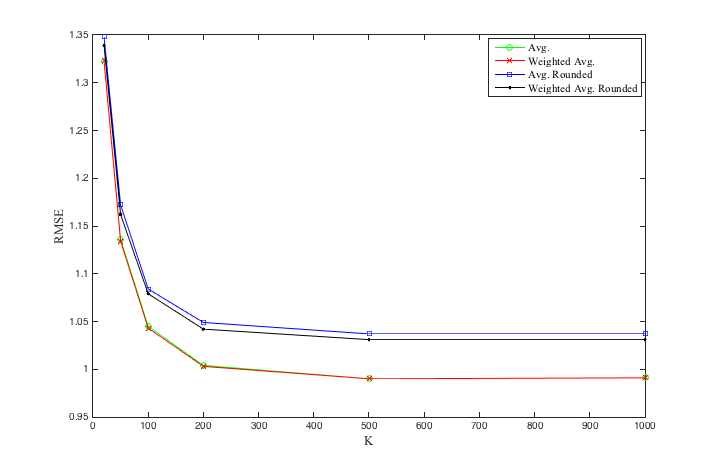
\includegraphics[width=0.8\textwidth]{images/rmse.png}
  \caption{RMSE for our collaborative filtering approach using
    different $K$ values}
  \label{fig:rmse}
\end{figure}

\begin{figure}[!ht]
  \centering 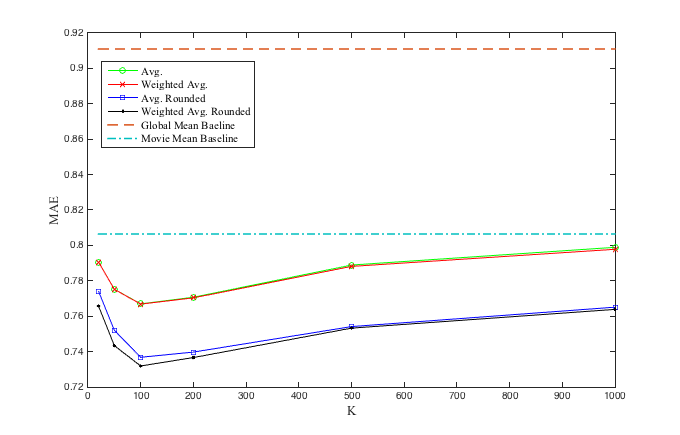
\includegraphics[width=0.8\textwidth]{images/MAE.png}
  \caption{MAE for our collaborative filtering approach using
    different $K$ values}
  \label{fig:mae}
\end{figure}

\begin{figure}[!ht]
  \centering 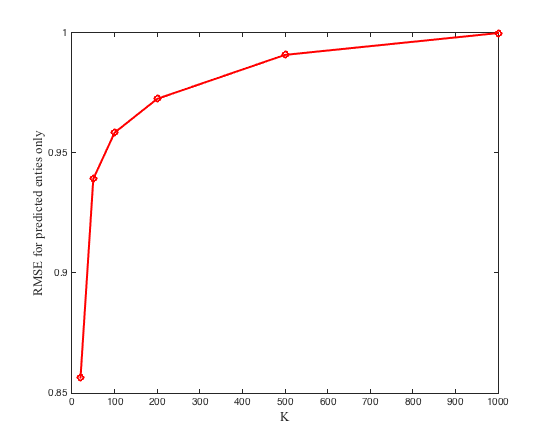
\includegraphics[width=0.8\textwidth]{images/rmsep.png}
  \caption{RMSE using weighted average prediction for predicted entries
    only with different $K$ values}
  \label{fig:rmsepred}
\end{figure}

The results suggest that using weighted average rating is better than
using unweighted average rating by only a small margin. This is due to
the fact that the variance of cosine similarities between the top $K$
movies being rated by the same user is not large. The result also
shows that rounding the predicted ratings will damage the RMSE
measurement, since RMSE is sensitive to noises and will amplify small
errors. Therefore, we only report the unrounded results below.

%% Regarding, rounding
%% the predictions, it can be noticed that rounding reduces MAE while it
%% largely increases RMSE over the movie mean baseline as shown in Figure
%% \ref{fig:rmse} since RMSE is more sensitive than MAE to outliers. If
%% rounding goes on the wrong direction, RMSE would increase. Therefore,
%% we have used unrounded version of weighted average prediction for
%% further experiments.

Figure ~\ref{fig:perc} shows the percentage of unpredicted ratings as
we varies $K$. It shows that increasing $K$ will reduce the percentage
of unpredicted ratings, since considering more similar neighbours
(movies) would increase the probability of having some of these movies
rated by the tesing user. However, this benefit will be insignificant
when $K$ is already large. For example, the percentage of unpredicted
ratings only drops from $0.84\%$ to $0.824\%$ as we increase $K$ from
$500$ to $1000$. As discussed above, this benefit will be overwhelmed
by the large variance introduced by large $K$.

\begin{figure}[!ht]
  \centering 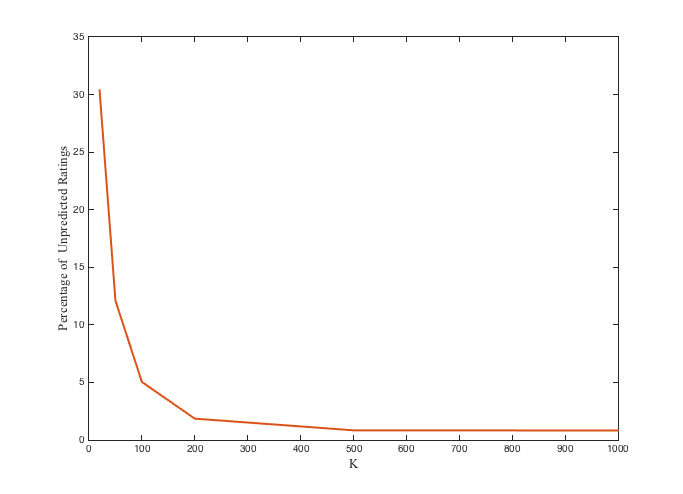
\includegraphics[width=0.8\textwidth]{images/perc.png}
  \caption{Percentage of unpredicted ratings using different $K$
    values}
  \label{fig:perc}
\end{figure}

%%Limiting m
To balance the ratio of predicted entries and the accuracy of
predicted ratings, we developed an adaptive prediction scheme. We use
two parameters to control the whole process: for a specific user $i$,
and movie $j$, we first find $K=500$ candidate movies using the above
algorithm. In the next step, instead of using all 500 similar movies,
we only use top $M$ movies that are rated by the user $i$. In the case
that the user $i$ rated less than $M$ movies among all $K=500$
candidates we use all candidates movies that are rated by user $i$.

%% However, our scheme aims at not sacrificing the accuracy of the
%% already predicted entries, the ones having many overlapping movies
%% that we can predict their ratings with using smaller $K$. Our scheme
%% is to use $K=500$ as it is the best point in terms of both accuracy
%% and percentage of missing ratings $0.84\%$, see Figure ~\ref{fig:rmse}
%% and Figure ~\ref{fig:mae}. However, we limit the number of neighbours
%% (similar movies) actually used in rating prediction to the top $M$ out
%% of these $K$ movies, where $M$ is much less than $K$.

Figure~\ref{fig:rmsem} and~\ref{fig:maem} show RMSE and MAE with
$K=500$ and varying $M$ from 5 to 100. With $M=20$ we are able to have
comparable accuracy as with $K=200$, while the comparable amount of
predicted entries as with $K=500$, See Table~\ref{tab:finres}.

%% It can be observed that having too small $M<20$
%% does not yield the best performance, we think the reason for that can
%% be that some of considered $K$ movies may have only one common user
%% rating them, having 1 cosine similarity, however, such movies with low
%% number of overlapped ratings may not be enough to have accurate
%% predictions. On the other hand increasing $M$ too much would increase
%% the error, this is reasonable and this is the motivation for using
%% $M$. Accordingly, we pick $M=20$, for our final predictions, which was
%% the best point for both Figure ~\ref{fig:rmsem} and ~\ref{fig:maem}.

\begin{figure}[!ht]
  \centering 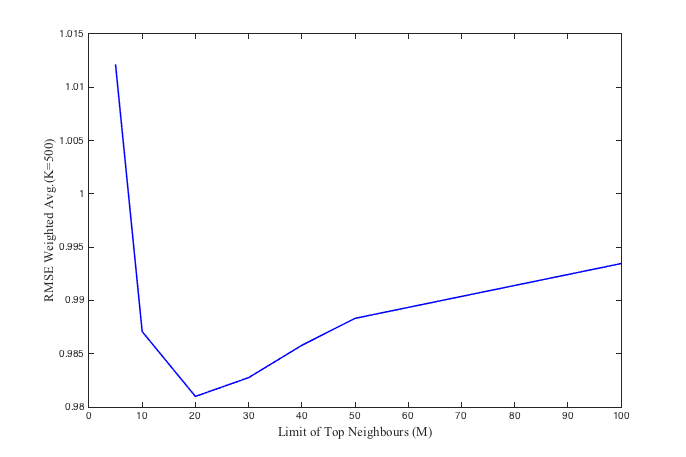
\includegraphics[width=0.8\textwidth]{images/rmsem.png}
  \caption{RMSE with varying $M$ using weighted average prediction and $K=500$.}
  \label{fig:rmsem}
\end{figure}

\begin{figure}[!ht]
  \centering 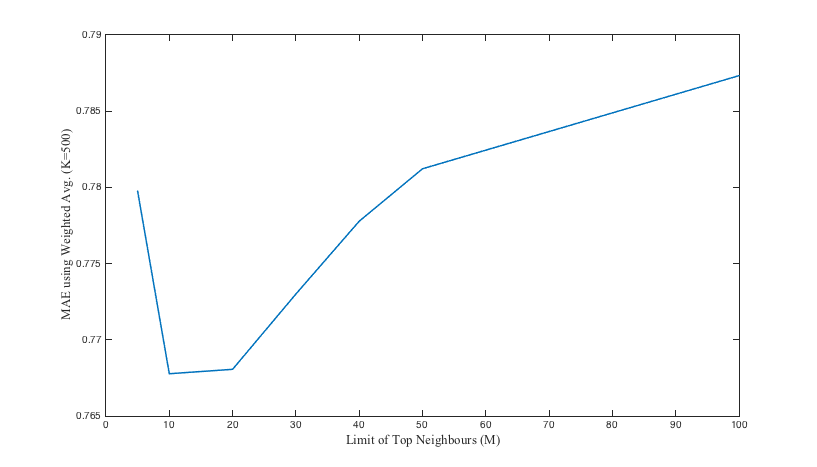
\includegraphics[width=0.8\textwidth]{images/MAEm.png}
  \caption{MAE with varying $M$ using weighted average prediction and $K=500$.}
  \label{fig:maem}
\end{figure}

%%FInal Results Table
Table \ref{tab:finres} summarizes our final results for our developed
collaborative filtering approach using $K=500$ and $M=20$. Results are
presented in terms of prediction accuracy using RMSE and MAE, and for
the percentage of unpredicted ratings. The table also shows the
comparison against two baselines methods: the global mean rating and
movie mean rating. Our collaborative filtering approach have better
accuracy than the two baselines with low percentage of unpredicted
entries.

\begin{table}[!ht]
  \centering
  \begin{tabular}{|c|c|c|c|c|}
    \hline & RMSE & MAE & Percentage of unpredicted ratings \\ \hline
    Collaborative Filtering & \textbf{0.98099} & \textbf{0.76806} &
    0.84\%\\ \hline Global Mean Baseline & 1.08502 & 0.91094 & -
    \\ \hline Movie Mean Baseline & 1.0067 & 0.8065 & - \\ \hline
  \end{tabular}
  \caption{Result of our collaborative filtering and the comparison
    against two baseline methods.}
  \label{tab:finres}
\end{table}


\textbf{Test on my own preference:} I selected 5 movies from
the training set and rated them as shown in Table
\ref{tab:preference}. To predict ratings for movies I
haven't rated, I put my ratings in the training set and
built a testing set containings all movies I haven't rated
associated with my own userID. Then I ran the same prediction script on the new
training set and testing set, and ranked the prediction
results in decreasing order of the predicted ratings. Movies
with highest predicted ratings include \textit{Teenage
  Catgirls in Heat}, \textit{The Gauntlet} and
\textit{Nevada Smith}. I think the prediction matches my
preference well as both \textit{The Gauntlet} and
\textit{Nevada Smith} are of same type with
\textit{Mississippi Burning} which I rated high.

\begin{table}[!ht]
  \centering
  \begin{tabular}{c c}
    Movie title & My rating \\
    \hline
    \textit{Catherine the Great} & 5.0 \\
    \textit{Me \& Isaac Newton} & 4.0 \\
    \textit{Mississippi Burning} & 5.0 \\
    \textit{Uptown Girls} & 4.0 \\
    \textit{The American President} & 5.0\\
  \end{tabular}
  \caption{My ratings for five movies in the training set.}
  \label{tab:preference}
\end{table}


  \section{Conclusion}

  % State the tasks of group members
\section*{Appendix A: group collboration}
Our group consists of four members. The tasks for each group member is listed below:
\begin{tabular}
  \centering
  \begin{table}{|c|c|
    \hline
    Dine Elreedy & Algorithm design, collaboarative filtering\\
    \hline
    Chen Liu & Algorithm design, collaboarative filtering, prediction\\
    \hline
    Hang Yan & Algorithm design, cloud platform\\
    \hline
    Hao Yan & Algorithm design, data analysis\\
    \hline
  \end{table}
  \caption{Tasks for group members}
  \label{tab:group}
\end{tabular}

\end{document}
